  \documentclass{article}
\usepackage[lecture]{preamble}
\usepackage{transparent}
\renewcommand{\O}{\mathcal{O}}

\title{CS 161 Lecture Notes}
\author{Mokhalad Aljuboori}
\date{Fall 2023 -- Inst. Peyrin Kao}



\definecolor{mygray}{rgb}{0.5,0.5,0.5}
\definecolor{othergray}{RGB}{192,192,192}
\lstset{
    basicstyle=\ttfamily,        % size of fonts used for the code
    breaklines=true,                 % automatic line breaking only at whitespace
    captionpos=b,                    % sets the caption-position to bottom
    escapeinside={\%*}{*},          % if you want to add LaTeX within your code
    language=C,
    frame=single,                % Add a frame around the code
    frameround=tttt,             % Round the frame corners
    rulecolor=\color{mygray},    % Color of the frame
    tabsize=4,
    backgroundcolor=\transparent{0.1}\color{othergray}  % choose the background color
}
% End
\newcommand{\xor}{\mathbin{\text{\scalebox{1.2}{$\oplus$}}}} % XOR operator, readjust size



\begin{document}
\maketitle

\lecture[08/23/23]{Introduction and Security Principles}

\subsection{Security Principles}
\subsubsection{Know your threat model}

\begin{definition}[Thread Model]
    A model of who your attacker is and what resources they have.
\end{definition}

Always assume the attacker can interact with systems without notice. Knows general information about systems (OS, vulnerabilities in software, etc). Assume the attacker is persistent and lucky.

\subsubsection{Consider Human Factors}
It all comes down to people.

For the users, if a security system is hard to use, users will find a way to subvert that system, compromising their system to make their lives easier.

For the programmers, they are likely to make mistakes, which are more frequent with some programming tools that others (C and C++ users make a lot of mistakes).

\subsubsection{Security is Economics}
The stronger the security, the more costly it will be. Therefore there should be a cost/benefit analyses to determine the security level we need. The expected benefit of your defense should be proportional to the expected cost of attack.

\subsubsection{Detect if you Can't Prevent}

{\color{red} TODO}
\begin{itemize}
    \item \textbf{Deterrence}: Stop the attack before it happens
    \item \textbf{Prevention}:
    \item \textbf{Detection}:
    \item \textbf{Response}:
\end{itemize}


\subsubsection{Detection in Depth}
An attacker should have to breach all defenses to successfully attack a system; Therefore, layer multiple types of defenses.

\subsubsection{Least Privilege}
Grant the minimum amount of access to applications/users needed to preform the tasks they need to do.

\subsubsection{Separation of Responsibility}
If you need to have a privilege, consider requiring multiple parties to work together to exercise it.

\begin{example}[Movie Theater Workers]
    Why is there two workers at the theaters that handle ticketing? One to give you the ticket and one to cut the ticket? This is a form of Separation of Responsibility to prevent insiders fraud.
\end{example}

\subsubsection{Shannon's Maxim}
Assume that the attackers knows your system. You should never reply on obscurity as part of your security. Always assume that the attacker knows every detail about the system you are working with (algorithms, hardware, defenses, etc.)

\subsubsection*{Design in Security from the Start}



%%%%%%%%%%%%%%%%%%%%%%%%%%%%%%%%%%%%%%%%%%%%%%%%%%%%%%%%%%%%%%%%%
%          Lecture 2:
%%%%%%%%%%%%%%%%%%%%%%%%%%%%%%%%%%%%%%%%%%%%%%%%%%%%%%%%%%%%%%%%%
\lecture[08/24/23]{x86 Assembly and Call Stack}
\subsection{Terminology}
\begin{itemize}
    \item 1 nibble = 4 bits
    \item 1 byte = 8 bits
    \item 1 word = 32 bits (on a 32-bit architectures)
\end{itemize}
A "word" is the size of a pointer, which depends on your CPU architecture.

\subsection{Compiler, Assembler, Linker, Loader (CALL)}
There are four main steps in running a C program.
\begin{enumerate}
    \item The compiler translates your C code into assembly instruction.
    \item The Assembler translates the assembly instructions from the compiler into machine code.
    \item The linker resolves dependencies on external libraries. After the linker is finished linking external libraries, it outputs a binary executable of the program that you can run.
    \item When the user runs the executable, the loaders sets up an address space in memory and runs the machine code instructions in the executable.
\end{enumerate}

\subsection{C Memory Layout}
At runtime, the OS gives the program an address space to stare any state necessary for program execution. Each byte of memory has a unique address.
\begin{center} % Center the diagram in the middle of the page
    \begin{tikzpicture}
        % Stack Section
        \draw (0,4) rectangle (6,7) node[midway] {Stack};
        \draw[->, thick] (3, 7) -- (3, 6.2); % Arrow pointing down
        \node[left, rotate=35] at (0, 7) {0xFFFFFFFF}; % Address for Stack

        % Heap Section
        \draw (0,2) rectangle (6,4) node[midway] {Heap};
        \draw[->, thick] (3, 2) -- (3, 2.8); % Arrow pointing up

        % Static Section
        \draw (0,1) rectangle (6,2) node[midway] {Static};

        % Code Section
        \draw (0,0) rectangle (6,1) node[midway] {Code};
        \node[left, rotate=35] at (0, 0) {0x00000000}; % Address for Code
    \end{tikzpicture}
\end{center}

\begin{itemize}
    \item The stack stores local variables and other information associated with function calls. The stack starts at the highest address and "grows down."

    \item The heap is dynamically allocated memory using \lstinline{malloc} and freed with \lstinline{free}.As more and more memory is allocated, it grows upwards.

    \item The Data is where static variables, which are allocated when the program is started.

    \item The Code is where the program code (machine code) lies, also called "text".
\end{itemize}


\subsection{Registers}
In addition to the $2^{32}$ bytes of memory in the address space, there are also registers, which store memory directly on the CPU where Each register can store on word. There are three special x86 registers that are relevant for these notes.

\begin{itemize}
    \item \emph{eip} is the instruction pointer, and it stores the address of the machine instruction currently being executed. In RISC-V this register is called the PC.
    \item \emph{ebp} is the base pointer, and it stores the address of the top of the current stack frame.
    \item \emph{esp} is the stack pointer, and it stores the address of the bottom of the current stack frame. In RISC-V, this register is called the SP (stack pointer)
\end{itemize}


{\color{red} Question: Why is there an e at the start of these register name?}\\
The e stands for "extended" and indicates that we are using a 32-bit system (extended from the original 16-bit system).

    {\color{red} Question: why do we need a base pointer if the stack always start at the highest address 0xFF...}\\
base pointers change as you make function calls, which open new frames with it's own local variables.
\subsection{Stack: Pushing and popping}
The x86 \lstinline{push} instruction allocate additional space on the stack then store the value in the newly allocated space.

The x86 \lstinline{pop} instruction increment the \emph{esp} so that the popped value is now below the esp. \emph{Note that the value is not wiped away from memory, it will be below the esp, which is now in undefined memory.}

\subsection{Calling Convention}
This class uses the AT\&T x86 syntax. This means that the destination register comes last.

References to registers are preceded with a percent sign.

Immediates are preceded with a dollar sign (i.e. \$1, \$0x4, etc).

Memory references use parenthesis and can have immediate offsets; for example 12(\%esp) dereferences memory 12 bytes away above the address contained in ESP.

\subsection{x86 Function Calls}
When we call a function in x86, we need to update the values in all three registers we've discussed:
\begin{itemize}
    \item eip, the instruction pointer, is currently pointing at the instruction of the caller. It needs to be changed to point to the instruction of the callee.
    \item ebp and esp currently point to the top and bottom of the caller stack frame, respectively.
\end{itemize}

When returning from a function, the \emph{ESP}, \emph{EBP}, and \emph{EIP} must return to their old values.

Here are the steps of calling a function.

\begin{enumerate}
    \item Push the arguments onto the stack in reverse order.
    \item Push the current value of $eip$ on the stack, this value is called $rip$ of the callee, which stands for return instruction pointer
    \item Push the EBP on the stack. This value is sometimes called $sfp$ of the callee which stands for saved frame pointer.
    \item {\color{red} TODO...}
    \item Begin function execution
\end{enumerate}

{\color{red} Question: if ebp is moved below the arguments, how can we have access to them in the called function?}\\
{\color{red} Question: which function calls main? Do we save the rip and sfp of main?}

%%%%%%%%%%%%%%%%%%%%%%%%%%%%%%%%%%%%%%%%%%%%%%%%%%%%%%%%%%%%%%%%%
%          Lecture 3: Memory Safety Vulnerabilities
%%%%%%%%%%%%%%%%%%%%%%%%%%%%%%%%%%%%%%%%%%%%%%%%%%%%%%%%%%%%%%%%%
\lecture[08/30/23]{Memory Safety Vulnerabilities}
\subsection{Buffer Overflow Error}
A buffer overflow bug is one where the programmer fails to perform adequate bounds checks, triggering an out-of-bounds memory access that writes beyond the bounds of some memory region. Attackers can use these out-of-bounds memory accesses to corrupt the program's intended behavior.

\begin{example}[Buffer Overflow Attack]
    Here is a piece of code that uses the gets function. The gets function will write bytes until the input contains a newline (\lstinline{\n}), not when the end of the array is reached.
    \begin{lstlisting}[language=C]
        char buf[8];
        int authenticated = 0;
        void vulnerable() {
            gets(buf);
        }
    \end{lstlisting}

    In C, static memory is filled in the order that variables are defined, so authenticated is at a higher address in memory than buf.

    If the user units something like: 12345678\textbf{?}
    This will override what the variable \lstinline{authenticated} stores into whatever we want, allowing us to maybe have privileges we weren't suppose to.

    In general the user can override any variable that's defined under the variable inside the gets function (whatever gets is writing into.)
\end{example}

\subsection{Stack Smashing}
The most common kind of buffer overflow occurs on stack memory. What are some values on the stack an attacker can overflow?
\begin{itemize}
    \item Local variables
    \item function arguments
    \item sfp
    \item rip
\end{itemize}

Recall when returning from a program, the EIP is set to the value of the RIP saved on the stack in memory. Stack smashing can be used for malicious code injection.


\begin{example}[Overwriting the RIP]
    Consider this program:

    \begin{lstlisting}[language=C]
        void vulnerable(void) {
            char name[20];
            gets(name);
        }
    \end{lstlisting}
    Assume that the attacker wants to execute malicious instructions at address \lstinline{0xDEADBEEF.} The attacker should write a carefully-chosen input that will override the value written into RIP, which is 24 bytes away from \lstinline{name}.

    One of the inputs could be:
    \begin{lstlisting}[language=python]
    'A' * 24 +
    '\xEF\xBE\xAD\xDE'

    # Note \xEF denotes EF in hexadecimal.l
    \end{lstlisting}



\end{example}

{\color{red} Question: Is the x86 calling convention used everywhere or is it used only in this class? If not how do we know what the stack looks like and where rip is.?} GDB


\subsection{Putting Together an Attack}
\begin{enumerate}
    \item Find a memory safety vulnerability
    \item write malicious shellcode at an known memory address
    \item overwrite the RIP with the address of the shellcode
    \item return from the function begin executing the written malicious shellcode
\end{enumerate}

\begin{definition}[shellcode]
    Shellcode is a small piece of machine code typically written in assembly language that is designed to be injected and executed directly in a computer's memory. It's often used in the context of exploiting software vulnerabilities to gain unauthorized access to a computer system. Here are some key points about shellcode:
\end{definition}
For the code:
\begin{lstlisting}
    void vulnerable(void) {
        char name[20];
        gets(name);
    }
\end{lstlisting}
Here is what the stack could look like if we write the shellcode at the beginning of name, an the rest is garbage ('A').

\begin{figure}[h]
    \centering
    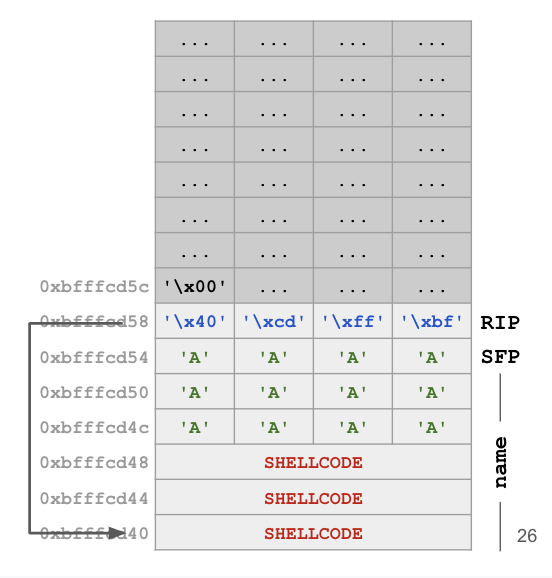
\includegraphics[scale=1.0]{images/writing-shellcode.png}
    \caption{The stack with shell code written at the beginning of name.}
\end{figure}


\subsection*{Writing Safer Code}
Realize that \lstinline{gets} is not safe. A safer function that reads input from the user is \lstinline{fgets} which requires the program to input exactly how many bites they could change.

In general, read up on the functions to see if they they have vulnerabilities in the \lstinline{man pages}


\subsection*{Integer Memory Safety Vulnerabilities}
This is an attacker where the attacker exploits how integers are represented in C memory.

Consider the program:
\begin{figure}[H]
    \begin{lstlisting}
        void function (int len, char * data) {
            char buf[64];
            if (len > 64) return;
            memcpy(buff, data, len);
        }
    \end{lstlisting}
\end{figure}

If we look at the function signature of memcpy: \\
\lstinline{void *memcpy(void* dest, const void *src, size_t n);} \\


\lecture[09/06/23]{More Memory Vulnerabilities}
\subsection{\lstinline{printf} vulnerabilities}

Consider the program:
\begin{lstlisting}
    void func(void) {
        int secret = 42;
        printf("%d\n");
    }
\end{lstlisting}
There is a mismatch between the format string specifiers and the arguments to printf. Printf expects a number to be in the second argument. So it will look 8 bytes above the rip of printf, to find the second argument (arguments are in reverse order).
The stack will look like this:
\begin{figure}[h]
    \centering
    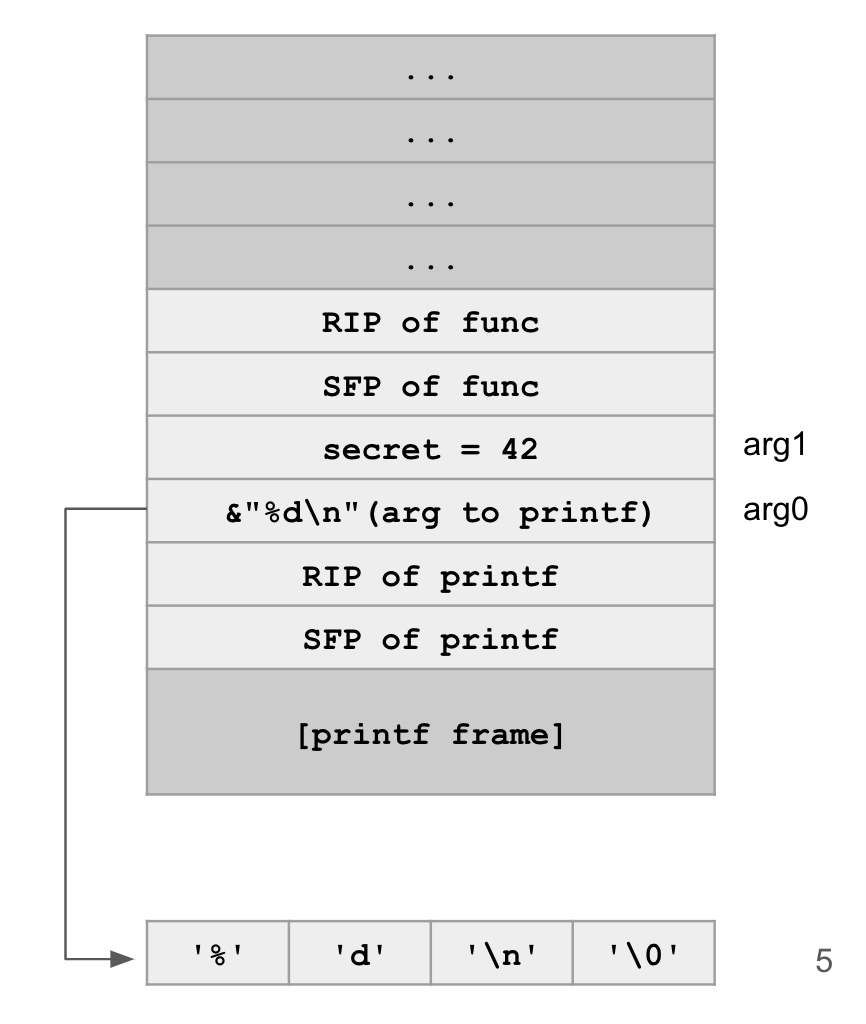
\includegraphics[scale=0.5]{images/printf-stack-vul.png}
    \caption{func(void) stack}
\end{figure}


You can also write values using the \lstinline{%n} specifier:

    \lstinline{%n} treats the next argument as a \textbf{pointer} and writes the number of bytes printed so far to that address (usually used to calculate output spacing)

\begin{example}[\%n example]
    Consider the program:
    \begin{lstlisting}
        void vulnerable(void) {
            char buf[16];
            char str[12];
            fgets(buf, 16, stdin);
            printf(buf);
        }
    \end{lstlisting}

    {\color{red} Question:} Construct an input to write 100 to address \lstinline{0xdeadbeef}

    \textbf{Solution:}
    \begin{center}
        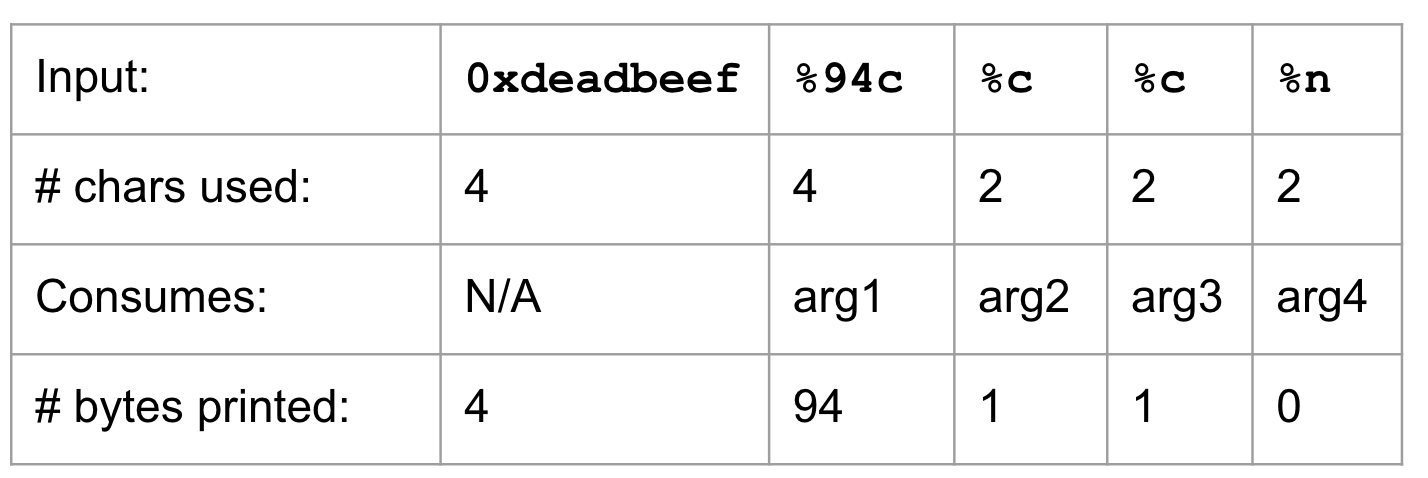
\includegraphics[scale=0.4]{images/solution-to-example-n.png} \\
    \end{center}
    Stack diagram:

    \begin{center}
        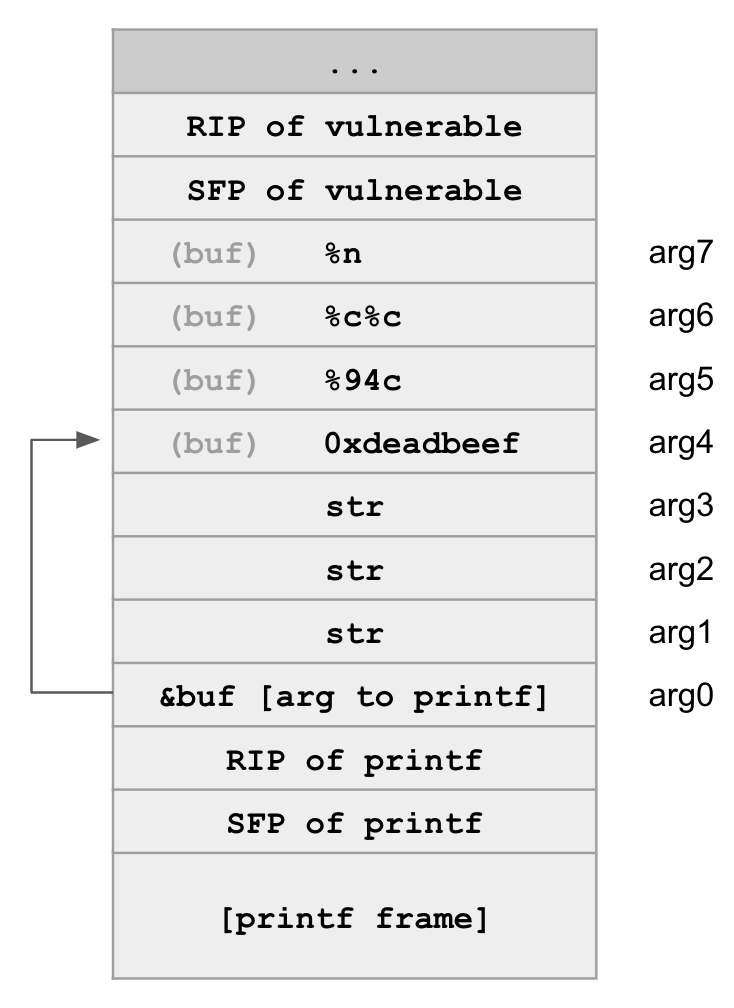
\includegraphics[scale=0.5]{images/example-n-stack-diagram.png}
    \end{center}
    Note \lstinline{%94c} prints the next argument on the stack as a character, padded to 94 bytes

\end{example}


\newpage
\subsubsection{Defense Against Printf Vulnerabilities}
Do not give the user control to the first argument of print f. Here is safe code
\begin{lstlisting}
    void not_vulnerable(void) {
        chat buf[64]
        if (fgets(buf, 64, stdin) == NULL)
            return;
        printf("%s", buf);
    }
\end{lstlisting}

\subsection{Off-by-one Vulnerabilities}
Consider the function:

\begin{lstlisting}
    void vulnerable(void) {
        char name[20];
        fread(name, 21, 1, stdin);
    }
\end{lstlisting}

\lstinline{name} holds 20 bytes, but we allow the attacker to write 21 bytes. Is it possible that an attacker could execute shellcode just by changing one byte?

The attacker is of course able to overwrite all 20 bytes of name, but also the least significant byte of the SFP of  vulnerable. If the

\lecture[09/11/23]{Mitigating Memory Safety Vulnerabilities}
\begin{enumerate}
    \item Using a memory-safe language. This is the only way to stop 100\% of memory safety vulnerabilities.
    \item Writing memory-safe code, like checking a ptr is not null before dereference. Using safe libraries.
\end{enumerate}
\subsection{Mitigation: Non-executable pages/ Write XOR Execute}
Common buffer overflow exploits involve the attacker placing shellcode somewhere in the stack and overwriting the rip to cause the program to execute that code. One way to defend against this category of attacks is to make some portions of memory non-executable, which means that data in these regions should not be interpreted as CPU instructions.

The code section of memory is executable but not writable. The stack is writable but not executable.

\subsection{Subverting Non-executable pages: Return into libc}
Most C programs import libraries with thousands or even millions lines of instructions, all of which are marked as executable. An attacker can exploit this by overwriting the rip to point to a desired C library function, and some take arguments. The attacker can carefully place the desired arguments to the library function on the stack.

\subsection{Subverting non-executable pages: Return-oriented programming}
We can construct a custom shellcode using pieces of code, called gadgets, that already exist in memory. These gadgets are not functions, they don't need to start with a prologue or end with an epilogue, just as long as they end with a \lstinline{ret} instruction. The general strategy for executing ROPs is to write a chain of return addresses at the RIP to achieve the behavior that we want. Each time we jump to an ROP gadget, we eventually execute the \lstinline{ret} instruction and then pop the next return address of the stack, jumping to the next gadget.

\subsection{Mitigation: Stack canaries}
a canary bird is a sacrificial animal commonly used by coal miners to alert when toxic gas builds up. We can use the same idea to prevent against buffer overflow attacks. The compiler places a canary value (stack canary) on the stack. This value is not used by the function so it should remain unchanged. After the function returns, if the cary value has changed, then it's like the canary bird died in the coal mine, so something must've gone wrong, so the program will crash before any further damage is done.

The stack canary is a random value generated at runtime. The canary is 1 world long. Stack canaries are usually guaranteed to contain a null byte (usually the first byte). This lets the canary defend against string-based memory safety exploits.

\subsection{Subverting Stack Canaries}
There are many exploits that the stack canary cannot detect:

\begin{itemize}
    \item Can't defend against attacks outside of the stack, like vulnerable heap memory.
    \item Stack canaries don't stop an attacker from overwriting local variables. Recall the \lstinline{authenticated} example.
    \item Some exploits do not write to non-consecutive parts of memory. For example, format string vulnerabilities let an attacker write directly to the rip without having to overwrite everything between a local variable and the rip, so the canary value is unchanged.
\end{itemize}


\lecture[9/11/23]{Intro to Cryptography}
Cryptography is the study of how to write secret messages. To formally study cryptography, we have to define a mathematically rigorous framework that lets us analyze the security of various cryptographic schemes.

\textbf{Meet Alice, Bob, Eve, and Mallory}. The most basic cryptography is one of ensuring the security of communications across an insecure medium. Alice and Bob wish to communicate thru a channel which insecure. The channel is subject to eavesdropping by Eve. In some settings, Eve may be replaced by an active adversary \emph{Mallory}, who can tamper with communications in addition to eavesdropping. The goal is for Alice and Bob to communicate in such a way that Eve has no clue about the contents of their exchange, and Mallory is unable to tamper with the contents of their exchange without being detected.

\begin{definition}[Key]
    The most basic building block of any cryptographic system is the key. It's a secret value that helps us secure messages. There are two main key models in modern cryptography:
    \begin{enumerate}
        \item  The \emph{symmetric key model}, Alice and Bob both know the value of a secret key, and must secure their communications using this shared secret value.
        \item The \emph{asymmetric key model}, each person has a secret key and a corresponding public key, recall RSA.
    \end{enumerate}
\end{definition}

In cryptography there are three main security properties/goals we want to achieve
\begin{enumerate}
    \item \textbf{Confidentiality}: The property that prevents adversaries from \textbf{reading} our private data.
    \item \textbf{Integrity}: The property that prevents adversaries from \textbf{tampering} with our private data without being detected.
    \item \textbf{Authenticity}: The property that lets us determine who created a given message.
\end{enumerate}
\subsubsection{Integrity (and Authenticity)}
Schemes provide integrity by adding a \textbf{tag} or \textbf{signature} on messages. Bob receives the message from Alice and checks if the tag/signature is valid. If it's not, then the authenticity of the message received is not guaranteed.

\begin{definition}[Kerckhoff's Security Principle]
    Cryptosystems should remain secure even when the attacker knows all internal details of the system. The key should be the only thing that must be kept secret, and the system should be designed to make it easy to change keys that are leaked (or suspected to be leaked). If your secrets are leaked, it is usually a lot easier to change the key than to replace every instance of the running software. (This principle is closely related to Shannon's Maxim: Don't rely on security through obscurity.)
\end{definition}
Consistent with Kerckhoff's principle, we will assume that the attacker knows the encryption and decryption algorithms. The only information the attacker is missing is the secret key(s).

Here is the model we'll be working with:
\begin{figure}[H]
    \centering
    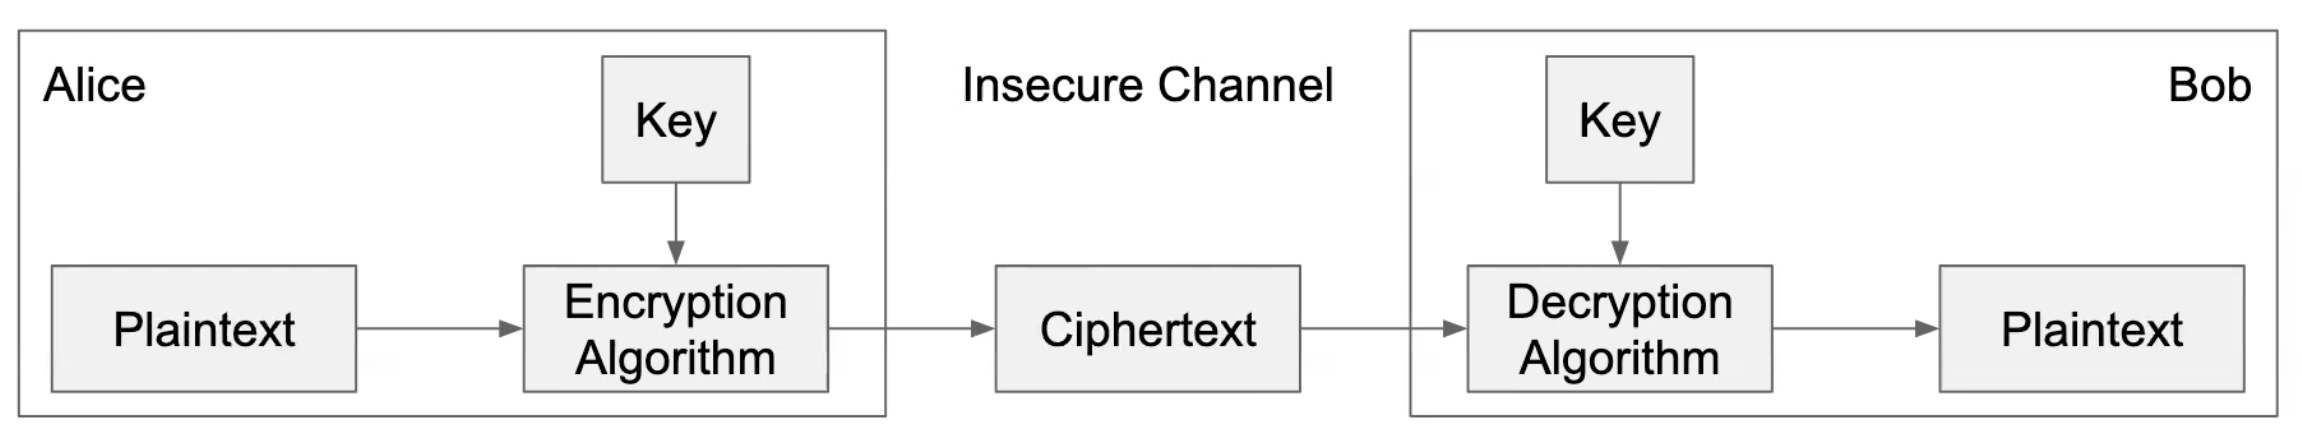
\includegraphics[scale=0.3]{images/crypto-comm-model.png}
    \caption{}
\end{figure}
\subsection{Threat Models}
When analyzing the confidentiality of an encryption scheme, there are several possibilities about how much access an eavesdropping attacker, Eve, has to the insecure channel.

\begin{itemize}
    \item \textbf{ciphertext-only attack}: Eve has intercepted a single encrypted message and wishes to recover the \textbf{plaintext} (the original message).
    \item \textbf{chosen-plaintext attack}: Eve can trick Alice to encrypt arbitrary messages of Eve’s choice, for which Eve can then observe the resulting ciphertext. (This might happen if Eve has access to the encryption system, or can generate external events that will lead Alice to sending predictable messages in response.) At some other point in time, Alice encrypts a message that is unknown to Eve; Eve intercepts the encryption of Alice’s message and aims to recover the message given what Eve has observed about previous encryptions.
\end{itemize}



\lecture[9/19/23]{Block Ciphers and Modes of Operation}
\subsection{Symmetric-Key Encryption}
A symmetric-key encryption scheme has three algorithms:
\begin{itemize}
    \item KeyGen() $\rightarrow K$: Generate a key $K$
    \item Enc($K, M$) $\rightarrow C$: Encrypt a \textbf{plaintext} $M$ using the key $K$  to produce \textbf{ciphertext} $C$.
    \item Dec($K, C$) $\rightarrow M$: Decrypt a ciphertext $C$ using the key $K$.
\end{itemize}

\begin{figure}[H]
    \centering
    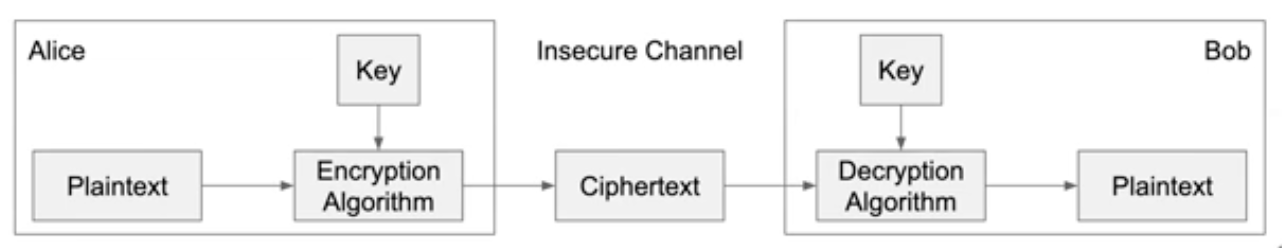
\includegraphics[scale=0.6]{images/symmetric-key-model.png}
    \caption{Symmetric Key Model}
\end{figure}

\subsubsection{Properties of Symmetric Encryption Scheme}
\begin{itemize}
    \item \textbf{correctness:} Decrypting a ciphertext should result in the message that was originally encrypted.
          \begin{itemize}
              \item $(\forall K, M) \; Dec(K, Enc(K, M)) = M$
          \end{itemize}
    \item Efficiency: Enc, Dec algorithms should be fast
    \item Security: confidentiality
\end{itemize}

\begin{definition}[Confidentiality]
    A more rigorous definition is as follows: the ciphertext $C$ should not give the attacker \emph{any additional information} about the plaintext message $M$.

    We can further formalize this definition by designing an experiment to test whether Eve has learned any additional information: if Eve can guess the ciphertext to be either any of $n$ messages, when Eve sees the ciphertext, the probability that Eve chooses the correct message is $1/n$, which is no different than if Eve hadn't seen the ciphertext at all.
\end{definition}

If we achieve confidentiality, meaning that; even though Eve can trick Alice into encrypting some messages, she still cannot distinguish whether Alice sent message $M_0$ or message $M_1$ in the experiment. This definition is known as \textbf{Indistinguishably under chosen plaintext attack (IND-CPA)}. We can use an experiment or game, played between the adversary Eve and the challenger Alice, to formally prove that a given encryption scheme is IND-CPA secure, or show that it is not IND-CPA secure.


\subsection{XOR Review}
Symmetric-key encryption often relies on the bitwise XOR operator (written as $\xor$). Here are some useful properties:
\begin{align*}
    x \xor 0          & = x                 &  & \text{0 is the identity}    \\
    x \xor x          & = 0                 &  & \text{x is its own inverse} \\
    x \xor y          & = y \xor x          &  & \text{commutative property} \\
    (x \xor y) \xor z & = x \xor (y \xor z) &  & \text{associative property}
\end{align*}

\subsection{One Time Pad; \emph{a symmetric encryption}}
The OTP scheme is a simple and idealized encryption scheme that helps illustrate some important concepts, though it is impractical for real-world use, as we'll see shortly.
In the one-time pad scheme, Alice and Bob share an $n$-bit secret key $K = k_1 \dots k_n$, generated every time Alice wants to encrypt a message, where each bit is picked uniformly at random.

Suppose Alice wishes to send the $n$-bit message $M= m_1\dots m_n$

The desired properties of the encryption scheme are:
\begin{enumerate}
    \item It should scramble up the message, i.e., map it a ciphertext $C = c_1 \dots c_n$
    \item Given knowledge of the secret key $K$, it should be easy to recover $M$ from $C$.
    \item Eve, who does not know $K$, should get \emph{no} information about $M$
\end{enumerate}
The algorithms for OTP are as follows:
\begin{itemize}
    \item $KeyGen()$, randomly generate an $n$-bit key.
    \item $Enc(K, M) = K \xor M \rightarrow$, the $j$th bit of the ciphertext is the $j$th bit of the message, XOR with the $j$th bit of the key.
    \item $Dec(K, C) = K \xor C$
\end{itemize}

\subsubsection{How Secure is OTP?}

If we were to reuse the same key for every encryption, we can show that this scheme is not secure: Eve would receive a ciphertext $C$ and trick Eve into encrypting $M_0$, if $C$ matches $M_0$, then Eve would guess $M_0$ is the message, otherwise, she guesses $M_1$. In summary, eve guesses the correct message with $100\%$ probability.

If we were to generate a random keys every time, we can show that this scheme is perfectly secure. However, random get generation is often expensive, and more over, when we generate the random key, we have to share this key with Bob in a secure way anyways, so why not send the message with this secure scheme.

\subsection{Block Ciphers}
Generating new keys for every encryption is difficult and expensive. Instead, Alice and Bob in most symmetric encryption schemes use a single key to repeatedly encrypt and decrypt messages. The block cipher is a fundamental building block in implementing such a symmetric scheme.

\begin{definition}[Block Cipher]
    An encryption/decryption algorithm that encrypts a fixed-size block of bits.\\
    \textbf{Properties:}
    \begin{itemize}
        \item \textbf{Correctness}: $E_k$ is a permutation (bijective function) on $n$-bit strings, $D_k$ is its inverse
        \item \textbf{Efficiency}: Encryption/decryption should be fast
        \item \textbf{Security}: The encryption function $E$ behaves like a random permutation.
    \end{itemize}
\end{definition}

\subsubsection{Security}
The block ciphers are not IND-CPA secure, because it's deterministic. No deterministic scheme can be IND-CPA secure because the adversary can always tell if the same message was encrypted twice. Moreover, another issue with block ciphers can only encrypt messages of a fixed size, usually 128-bit messages. We'll address these issues with \textbf{modes of operations}.

\subsection{Block Cipher Modes of Operation}
In order to support encrpytion of longer messages, we can split the message into multi 128 bits, and apply a block sipher to each substring, and then concatinating the ciphertext to obtain encrypted code.

\lecture[9/20/23]{Cryptographic Hashes and MACs}
\subsection{Cryptographic Hashes}
\begin{definition}[Hash Function]
    A cryptographic hash function is a function, $H$, that when applied on a message, $M$, can be used to generate a fixed-length "fingerprint" of the message. The hash function, $H$, is deterministic, meaning if you compute $H(M)$ twice with the same input $M$, you will always get the same hash value twice. The hash function is unkeyed.
\end{definition}

For hash functions, since the produce "finger prints", any change to the message, no matter how small, will change many of the bits of the hash value with there being no detectable patterns as to how the output changes based on specific input changes.

\subsubsection{Properties of Hash Functions}
Some of the most significant properties include the following
\begin{itemize}
    \item \textbf{One-way}: Given $x$, it is easy to compute $H(x)$. However, given a hash value $y$, it is unfeasible to find any input $x$ such that $H(x) = y$. This is also known as $pre=image resistant$.
    \item \textbf{Second Preimage Resistant}: Given $x$, it is infeasible to find another input $x^\prime$ such that $x \neq x^\prime$ but $H(x) = H(x^\prime)$
    \item \textbf{Collision Resistant}: It's infeasible to find \emph{any pair of messages} $x, x^\prime$ such that $x \neq x^\prime$ but $H(x) = H(x^\prime)$. This is very similar to the second property but now the adversary can freely choose their starting point $x$.
\end{itemize}

\textbf{Note:} "infeasible" means that there is no known way to accomplish it with any realistic amount of computing power. Also the third property implies the second.

\subsubsection{Hash Algorithms}
Today there are two primary "families" of hash algorithms in common use that are believed to be secure: SHA2 and SHA3. The only significant different is that SHA2 is vulnerable to a \emph{length extension attack}.

\subsubsection{Do Hashes provide integrity}
It depends on your threat model. If Alice wants to communicate with Bob over an insecure channel where Mallory is capable or tampering with the message, hashes do not provide integrity. Mallory can simply change the message and the hash value so that when bob checks the hash of the tampered message recieved and the hash of the tampered message, it will be the same even though the message is tampered with.

This is because there is no key, no secrecy to the hash function. Anyone can compute the hash of a message. But can we use hash functions as a building blocks? Yes in MACs,
\subsection{Message Authentication Codes}
MACS guarantee integrity and authenticity to enable the recipient of a message to detect spoofing and tampering.
\begin{definition}
    A MAC (message authentication code) is a keyed (takes in a secret key) checksum of the message that is sent along with the message. It takes a fixed-length secret key and an arbitrary-length message, and outputs a fixed-length checksum. A secure MAC has the property that \textbf{any change to the message will render the checksum invalid.} Formally, the MAC, $T$, on a message $M$, is a value $F(K,M) = T$, called the tag for $M$ or the MAC of $M$.
\end{definition}

When Alice wants to send a message with integrity and authentication, she first computes a MAC on the message $T_{ag} = \text{MAC}(K, M)$. She sends the message and the mac $\langle M, T_{ag}\rangle$. When bob recieves the message, he will recompute $\text{MAC}(K, M)$ and check that it makes the tag he received. If the tags don't match, he will ignore the message and presume that some tampering or message corruption occurred.

\begin{figure}[H]
    \centering
    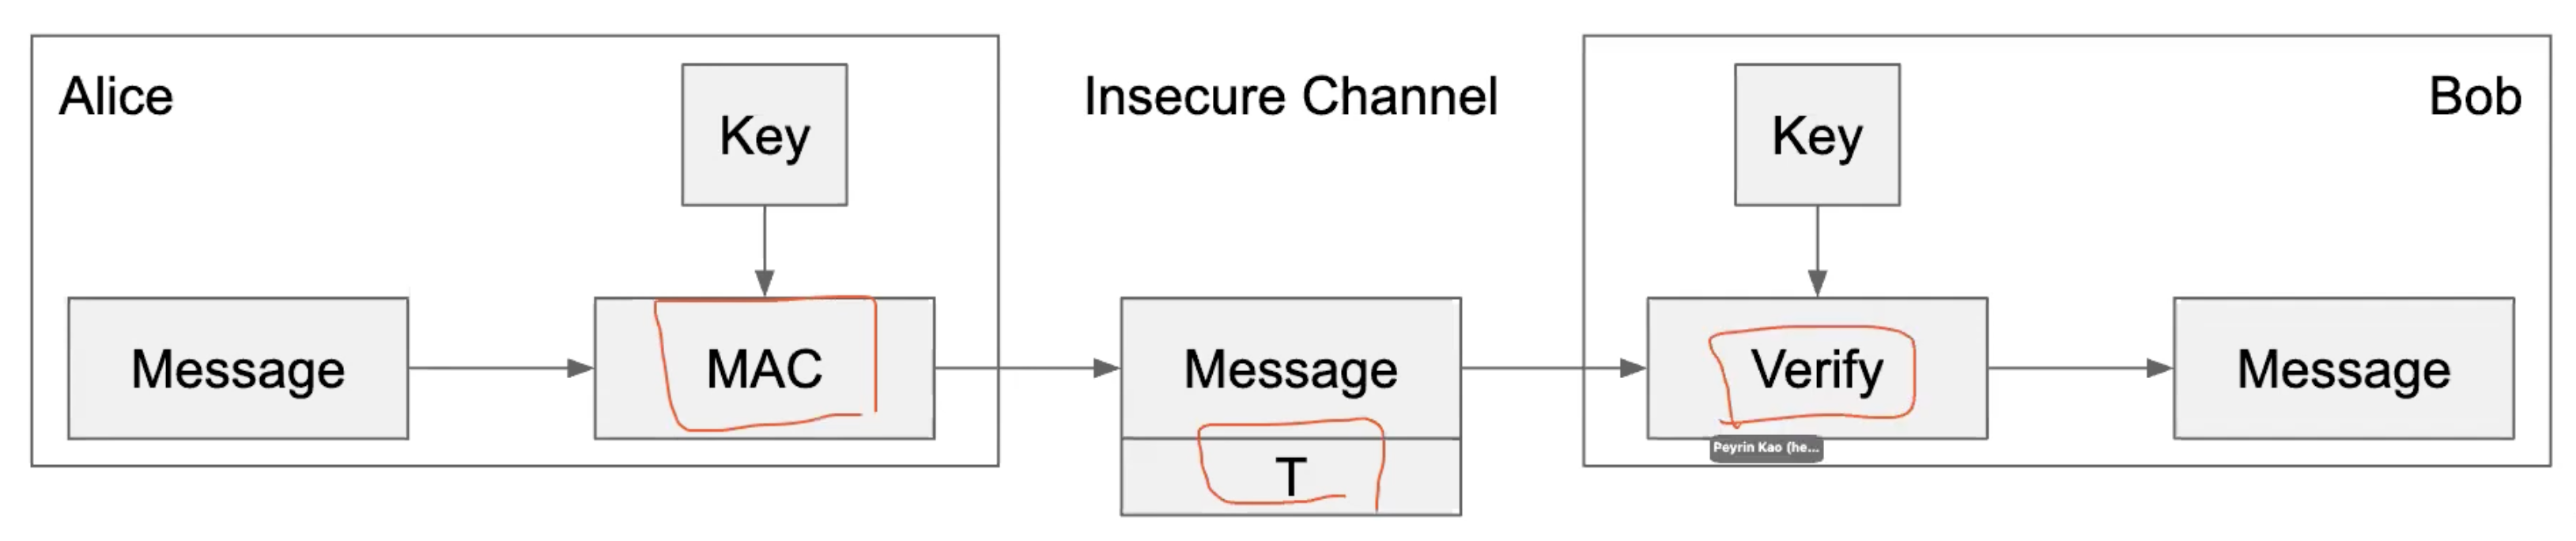
\includegraphics[scale=.28]{images/macs.png}
    \caption{}
\end{figure}

\subsection{AES-EMAC}
How do we build secure MACs? There are multiple schemes out there but a good on is AES-CMAC, an algorithm standardized by NIST. But lets look at AES-EMAC; it is a slightly simplified version of AES-CMAC that retains its essential character but differs in a few details.

In AES-EMAC, the key $K$ is 256 bits, viewed as a pair of 128-bit AES keys: $K = \langle K_1, K_2 \rangle$.

    {\color{red} What are AES keys?}

The message $M$ is decomposed into a sequence of 128-bit blocks:

\end{document}

